\documentclass[pdflatex,sn-mathphys-num]{sn-jnl}
\usepackage{graphicx}
\usepackage{booktabs}
\usepackage{amsmath,amssymb}
\usepackage{orcidlink}
\renewcommand{\orcid}[1]{~\orcidlink{#1}}
\begin{document}

\title[FABRID-IDS]{FABRID-IDS: Federated Alert-Budget Reallocation for Heterogeneous IoT Intrusion Detection}
\author*[1]{\fnm{Salaheddine} \sur{Naslouby}\orcid{0009-0002-7295-7816}}\email{naslouby.salahe@gmail.com}
\author[2]{\fnm{Mohamed} \sur{Lachgar}}\email{m.lachgar@uca.ac.ma}
\author[1]{\fnm{Hamid} \sur{Hrimech}}\email{hamid.hrimech@uhp.ac.ma}
\affil[1]{\orgname{Hassan First University}, \orgdiv{National School of Applied Sciences (ENSA), LAMSAD Laboratory}, \orgaddress{\city{Berrechid}, \country{Morocco}}}
\affil[2]{\orgname{Cadi Ayyad University}, \orgdiv{Higher Normal School (ENS), L2IS Laboratory}, \orgaddress{\city{Marrakech}, \country{Morocco}}}

\abstract{A frozen federated anomaly scorer can rank attacks well while still producing unreliable operating thresholds across heterogeneous clients. FABRID-IDS treats post-training threshold selection as federated alert-budget reallocation: client-specific nominal false-positive-rate (FPR) targets are assigned under a shared weighted budget and then calibrated independently on local benign data. The primary evaluation uses nine N-BaIoT devices, ten detector seeds, and five nominal budgets; CIC IoT-DIAD provides a secondary protocol stress test with different clients, features, and a different scorer. At $B=0.001$, unrestricted Macro and Tail allocations realize a federation FPR of $0.00170$, or $1.696B$, despite satisfying the nominal allocation constraint. Conservative calibration reduces the realized FPR to $0.00036$ but lowers macro recall from $0.3778$ to $0.2445$ and does not restore worst-client recall. Mean AUROC and AUPRC are $0.9995$ and $0.9999$, yet FABRID-family minimum-client recall remains zero across the evaluated N-BaIoT budgets. Thus, satisfying the nominal federation-level alert-budget constraint does not guarantee the realized FPR or client-level detection behavior after finite local calibration, even when score ranking is near perfect.}
\keywords{federated intrusion detection, Internet of Things, alert-budget reallocation, false-positive-rate constraint, threshold calibration}
\maketitle

\section{Introduction}\label{sec:introduction}
Federated IoT detection distributes model training across clients, but deployment still requires a threshold that converts anomaly scores into alerts \cite{nguyen2019diot,wang2021noniid,hamdi2023flids}. Shared and client-specific thresholding have been studied \cite{laridi2024threshold,Asiri2025Decentralized,Khan2026FedDTCN}, yet neither determines how a federation-wide FPR budget should be divided across heterogeneous clients. With a frozen scorer, differences in benign-score distributions and attack-recall curves can produce uneven false-alarm and detection-utility outcomes across clients.

FABRID-IDS treats this as alert-budget reallocation. Given a fixed scorer, it selects client-specific nominal rates $\alpha_k$ under the federation constraint $\sum_k w_k \alpha_k \leq B$, recalibrates thresholds on disjoint benign data, and evaluates them on held-out records. $B$ is a nominal federation-level FPR budget, not a realized-FPR guarantee.

The contributions are federation-constrained alert-budget allocation, a frozen-scorer protocol separating allocation, calibration, and testing, and paired N-BaIoT evidence that nominal compliance need not preserve realized FPR or worst-client recall.

The rest of the paper covers related work, methods, results, and implications.

\section{Related work and scope}\label{sec:related}
Federated IoT IDS research has mainly focused on detector training \cite{nguyen2019diot,wang2021noniid,hamdi2023flids,mcmahan2017fedavg}, while threshold regulation and distributed anomaly detection address related operating-point questions \cite{bridges2017threshold,ochiai2023global}. Laridi et al. \cite{laridi2024threshold} aggregate client summary statistics into one global anomaly threshold. Asiri et al. \cite{Asiri2025Decentralized} compute local 95th-percentile benign reconstruction-error thresholds and average them into one global threshold. Fed-DTCN \cite{Khan2026FedDTCN} uses held-out benign calibration data to select client-specific thresholds for target local FPRs. These designs neither jointly allocate client-specific nominal FPR targets under one federation-level budget nor formulate a finite-sample guarantee for the resulting realized federation FPR.

Rate-constrained and Neyman-Pearson methods address explicit error-rate control \cite{kumar2021implicit,tong2018np}, while federated and conformal calibration provide finite-sample control under stated sampling or exchangeability assumptions \cite{lu2023fcp,angelopoulos2024conformalrisk}. FABRID-IDS jointly selects client-specific nominal rates under $\sum_k w_k \alpha_k \leq B$, recalibrates thresholds on disjoint benign data, and evaluates realized federation and client-level FPR. The federation-level allocation formulation is the contribution; CVaR, order statistics, mixed-integer optimization, and finite-sample calibration are established components. Because N-BaIoT is split by released source order, the splits establish neither deployment chronology nor exchangeability.

\section{FABRID-IDS}\label{sec:method}
\subsection{Protocol and utility}
For $K$ clients, a frozen scorer $s_k(\cdot)$ produces anomaly scores. Released source order defines benign training (50\%), frontier (20\%), final-calibration (10\%), and test (20\%) splits; the initial 20\% of each retained attack subtype forms the validation split and the remainder forms the test split. The pipeline proceeds through training, frozen scoring, frontier utility estimation, allocation, final calibration, and testing; final-calibration and test benign records are not allocation inputs.

For ascending benign scores $x_{(1)},\ldots,x_{(n)}$ and nominal target $\alpha$, threshold calibration uses a standard order-statistic construction \cite{angelopoulos2024conformalrisk}
\begin{equation}
 \tau(\alpha)=x_{(r)},\qquad r=\left\lceil(n+1)(1-\alpha)\right\rceil,
 \label{eq:orderstat}
\end{equation}
with $\tau=+\infty$ if $\alpha\leq0$, $n=0$, or $r>n$; alerts require $s>\tau$. Frontier utility $u_k(\alpha)$ is the mean recall across attack subtypes. Allocation utility is estimated from labeled attack validation data; only the subsequent final threshold calibration uses benign data. The evaluated procedure is therefore attack-informed alert-budget reallocation rather than label-free deployment adaptation. Eligible subtypes require at least 50 validation rows, clients require at least 200 rows across two subtypes, and the 207-point grid spans $[0,0.05]$ and includes every evaluated budget.

\subsection{Allocation and calibration}
FABRID-IDS reallocates the nominal alert budget by selecting client-specific grid rates subject to
\begin{equation}
 \sum_{k=1}^{K} w_k\alpha_k\leq B. \label{eq:budget}
\end{equation}
Primary N-BaIoT results use $w_k=1/K$, so nominal and realized federation FPR are both equal-client averages. One-hot mixed-integer programs (HiGHS) maximize mean $u_k$ (Macro) or lower-tail CVaR at quantile 0.25 (Tail) \cite{rockafellar2000cvar}. For nine clients, the Tail objective averages the three lowest utilities. Tail optimizes lower-tail CVaR at the stated quantile, whereas minimum-client recall is reported separately as a stricter worst-client stress endpoint. Candidate frontier rates below twice the order-statistic transition are excluded.

Final thresholds are recalibrated with Eq.~\eqref{eq:orderstat}. The conservative intervention selects the smallest rank satisfying the binomial calibration construction \cite{angelopoulos2024conformalrisk}
\begin{equation}
 r_{.95}=\min\{r:\Pr[\mathrm{Binomial}(n,1-\alpha)\leq r-1]\geq0.95\}.
 \label{eq:conservative}
\end{equation}
The resulting threshold retains the strict $s>\tau$ alert rule. This rank adjustment is used as a finite-sample sensitivity intervention rather than as a deployment guarantee under the source-order split. Its nominal 95\% interpretation requires the calibration data and future benign observations to satisfy the stated i.i.d. assumption.

With strict alerts, $\alpha<2/(n+1)$ gives either $r>n$ or a maximum-score threshold and zero calibration alerts; the smallest nonzero empirical FPR is $1/n$ (absent ties). Rates below this transition cannot generate a nonzero empirical calibration FPR under strict thresholding; excluding them prevents the optimizer from assigning nominal budget to grid points that are empirically indistinguishable from a zero-alert calibration point. Ecobee has $n=1311$ on the final-calibration split, so targets below $0.001524$ calibrate to zero alerts. This calculation explains why sufficiently small allocated rates produce no calibration alerts, but it does not explain the subsequent held-out FPR shift.

\subsection{Frozen scorer}
The primary scorer is the maximum of frozen frontier-reference percentile ranks for autoencoder reconstruction error and the mean of the jitter-based temporal feature \texttt{HH\_jit\_L0.1\_mean}, denoted $f_{75}$. The $f_{75}$ candidate and scorer ablations were predeclared for development-only selection. The autoencoder uses [64,16] layers, ten rounds of three local epochs, row-count-weighted averaging, Adam (0.001), batch size 64, MSE, and per-client training-split normalization; ten detector seeds are the paired replication unit.

\section{Experimental methodology}\label{sec:experiments}
The primary experiment uses nine N-BaIoT devices and five prespecified budgets from $B=0.001$ through $B=0.020$ (Table~\ref{tab:primary}). Macro recall is the mean of client-level macro recalls, each computed over eligible attack subtypes; minimum-client recall is their minimum.

Prespecified contrasts compare Macro with Equal-FPR on macro recall and Tail with Equal-FPR on minimum-client recall using ten paired seeds, exact sign-flip tests, 50,000-resample paired-bootstrap CIs, and Holm correction over each five-budget family. CIC IoT-DIAD provides a 19-client secondary protocol stress test using 57 features and reconstruction error alone. Because the client population, feature representation, and scorer all change, the experiment is not used for cross-dataset mechanism attribution.

\section{Results}\label{sec:results}
\subsection{Nominal and realized operating points}
At $B=0.001$, unrestricted Macro and Tail each realize federation FPR $0.00170$ ($1.696B$), whereas their conservative variants realize $0.00036$ ($0.358B$) and macro recall falls from $0.3778$ to $0.2445$. At $B=0.005$, Macro realizes $0.706B$ with recall $0.4644$, while Tail realizes $1.290B$ with recall $0.4977$. These same-$B$ comparisons hold nominal alert-budget expenditure fixed rather than realized FPR. The optimizer constrains $\sum_k w_k\alpha_k$, whereas evaluation measures the FPR produced after independent local calibration. The observed divergence shows that nominal budget compliance can coexist with federation-level overshoot or undershoot and different detection utility.

\begin{figure}[!t]
\centering
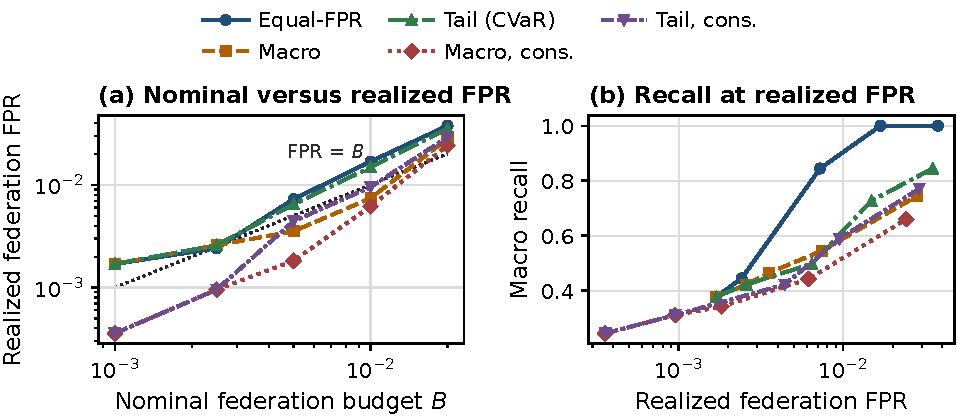
\includegraphics[width=0.8\textwidth]{realized_fpr_lines.pdf}
\caption{N-BaIoT means across ten detector seeds. (a) Nominal federation alert budget $B$ against realized equal-client federation FPR; the diagonal marks equality. (b) Macro recall at each observed realized federation FPR. Lines connect evaluated operating points only.}
\label{fig:realized}
\end{figure}

\begin{table}[!b]
\caption{N-BaIoT means across ten detector seeds: macro recall and realized federation FPR divided by nominal budget. Minimum-client recall is zero for every FABRID-family policy--budget cell.}
\label{tab:primary}
\centering
\small
\renewcommand{\arraystretch}{1.00}
\begin{tabular*}{\textwidth}{@{\extracolsep{\fill}}lccccc@{}}
\toprule
$B$ & Equal-FPR & Macro & Tail & Macro, cons. & Tail, cons.\\
\midrule
\multicolumn{6}{@{}l}{\textit{(a) Macro recall}}\\
0.0010 & 0.3778 & 0.3778 & 0.3778 & 0.2445 & 0.2445\\
0.0025 & 0.4445 & 0.4222 & 0.4222 & 0.3111 & 0.3111\\
0.0050 & 0.8444 & 0.4644 & 0.4977 & 0.3422 & 0.4222\\
0.0100 & 0.9999 & 0.5444 & 0.7266 & 0.4422 & 0.5889\\
0.0200 & 1.0000 & 0.7444 & 0.8444 & 0.6600 & 0.7711\\
\midrule
\multicolumn{6}{@{}l}{\textit{(b) Realized FPR$/B$}}\\
0.0010 & 1.70 & 1.70 & 1.70 & 0.36 & 0.36\\
0.0025 & 0.97 & 1.03 & 1.03 & 0.38 & 0.38\\
0.0050 & 1.45 & 0.71 & 1.29 & 0.36 & 0.88\\
0.0100 & 1.68 & 0.74 & 1.48 & 0.62 & 0.95\\
0.0200 & 1.88 & 1.40 & 1.75 & 1.21 & 1.45\\
\bottomrule
\end{tabular*}
\end{table}

\begin{figure}[!t]
\centering
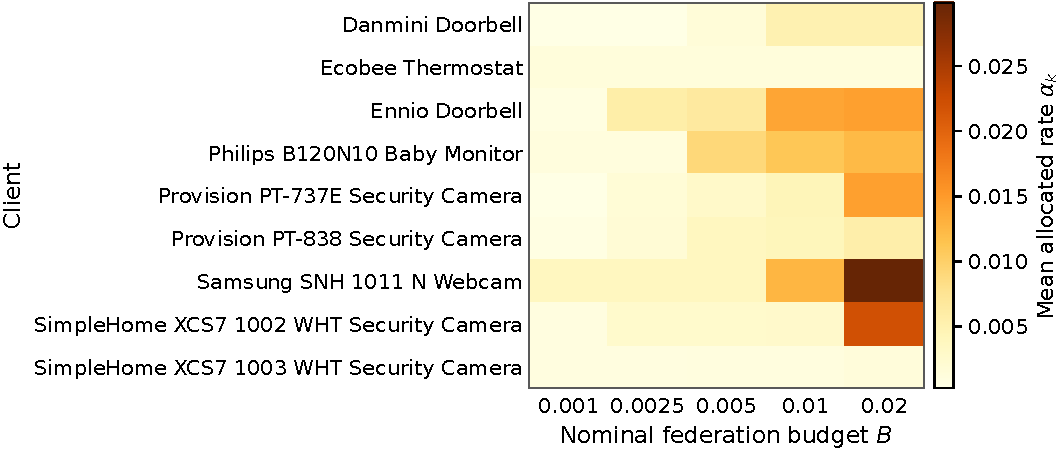
\includegraphics[width=0.85\textwidth]{macro_allocation_heatmap.pdf}
\caption{Mean Macro-policy client-specific nominal rates $\alpha_k$ across ten N-BaIoT detector seeds. Each column satisfies $\sum_k w_k\alpha_k\leq B$. Across 500 resamples of the frontier and attack-validation scores, selected client rates change in 77.8--84.9\% of replicates across budgets; the heatmap therefore summarizes mean allocation patterns rather than stable client-specific operating points.}
\label{fig:allocation}
\end{figure}

\subsection{Tail objective and worst-client behavior}
Tail optimizes lower-tail CVaR, but minimum-client recall is zero for every FABRID policy--budget cell and cannot distinguish unrestricted Macro and Tail. Danmini\_Doorbell is the persistent worst-client case: its macro attack recall, final-calibration benign FPR, and held-out benign FPR are all zero in all 100 unrestricted-policy--seed--budget cells. With $n=4955$ benign final-calibration records, its zero-alert transition is $2/(n+1)=0.000404$; its allocated-rate range crosses this finite-sample transition.

Ecobee illustrates a different calibration/test discrepancy. At $B=0.020$, Macro assigns mean $\alpha_k=0.001164$, below $2/(1311+1)$; its final-calibration FPR is therefore zero, while mean held-out benign FPR is $0.006672$ and recall is $0.6000$. Finite calibration resolution explains the zero-alert calibration point, but the experiment cannot separate that effect from distributional differences between the source-order final-calibration and test partitions.

\subsection{Primary contrasts and ranking ceiling}
Macro and Equal-FPR are identical at $B=0.001$; their $-0.0222$ difference at $B=0.0025$ is not statistically distinguishable from zero, and Macro recall is lower at larger budgets. Tail and Equal-FPR have identical minimum-client recall through $B=0.005$; Equal-FPR is higher at the two larger budgets (Table~\ref{tab:contrasts}).

\begin{table}[!t]
\caption{Prespecified paired seed-level contrasts ($n=10$): 50,000 paired-bootstrap CIs and Holm-adjusted exact paired sign-flip $p$ values over the five-budget family.}
\label{tab:contrasts}
\centering
\small
\renewcommand{\arraystretch}{1.00}
\begin{tabular*}{0.88\textwidth}{@{\extracolsep{\fill}}lccc@{}}
\toprule
$B$ & Mean $\Delta$ & 95\% CI & Holm $p$\\
\midrule
\multicolumn{4}{@{}l}{\textit{Macro $-$ Equal-FPR, macro recall}}\\
0.0010 & 0.0000 & [0.0000, 0.0000] & 1.0000\\
0.0025 & $-$0.0222 & [$-$0.0556, 0.0111] & 0.3594\\
0.0050 & $-$0.3800 & [$-$0.4133, $-$0.3466] & 0.0098\\
0.0100 & $-$0.4555 & [$-$0.5000, $-$0.4111] & 0.0098\\
0.0200 & $-$0.2556 & [$-$0.2889, $-$0.2222] & 0.0098\\
\midrule
\multicolumn{4}{@{}l}{\textit{Tail $-$ Equal-FPR, minimum-client recall}}\\
0.0010 & 0.0000 & [0.0000, 0.0000] & 1.0000\\
0.0025 & 0.0000 & [0.0000, 0.0000] & 1.0000\\
0.0050 & 0.0000 & [0.0000, 0.0000] & 1.0000\\
0.0100 & $-$0.9998 & [$-$0.9998, $-$0.9998] & 0.0098\\
0.0200 & $-$0.9999 & [$-$0.9999, $-$0.9999] & 0.0098\\
\bottomrule
\end{tabular*}
\end{table}

Because allocation changes thresholds rather than anomaly scores, AUROC and AUPRC are policy-invariant by construction. Their mean values are $0.9995$ and $0.9999$, respectively, yet FABRID-family minimum-client recall remains zero across all five N-BaIoT budgets. Near-perfect ranking metrics therefore do not imply reliable worst-client behavior at the evaluated low-FPR operating points.

\subsection{Secondary protocol stress test}
CIC IoT-DIAD provides a secondary protocol stress test. Across the five nominal budgets, macro recall ranges from $0.3614$ to $0.5016$, realized federation FPR from $0.0098$ to $0.0311$, and minimum-client recall from $0.0000$ to $0.0251$. The nominal-to-realized mismatch therefore remains visible under this second protocol, but different clients, features, and reconstruction-error-only scoring prevent attribution to the same mechanism as in N-BaIoT.

\begin{table}[!t]
\caption{CIC IoT-DIAD secondary protocol stress test: 19 clients, ten seeds, equal-client weighting, and reconstruction-error scoring.}
\label{tab:external}
\centering
\renewcommand{\arraystretch}{1.00}
\begin{tabular*}{0.82\textwidth}{@{\extracolsep{\fill}}lccc@{}}
\toprule
$B$ & Macro recall & Minimum-client recall & Realized FPR\\
\midrule
0.0010 & 0.3614 & 0.0000 & 0.0098\\
0.0025 & 0.3970 & 0.0000 & 0.0118\\
0.0050 & 0.4318 & 0.0007 & 0.0160\\
0.0100 & 0.4602 & 0.0089 & 0.0213\\
0.0200 & 0.5016 & 0.0251 & 0.0311\\
\bottomrule
\end{tabular*}
\end{table}

\section{Discussion}\label{sec:discussion}
On N-BaIoT, nominal budget feasibility does not imply realized budget fidelity. At $B=0.001$, unrestricted policies realize $1.696B$; conservative calibration lowers realized FPR and recall without recovering Danmini Doorbell detection. Equal-FPR achieves higher macro recall at several budgets, so the evidence does not support uniform superiority of any allocation policy.

Finite calibration granularity can force zero-alert points, as for Ecobee, but the source-order split cannot separate this effect from calibration/test distribution differences and does not establish temporal drift. Attack-informed utility shows limited transfer in family-disjoint stress tests, which remain within-benchmark rather than evidence of OOD generalization.

Evidence is limited to one scorer, nine devices, ten seeds, five budgets, and the CIC IoT-DIAD stress test. Privacy, adversarial clients, deployment overhead, and scorer-level remedies are outside scope.

\section{Conclusion}\label{sec:conclusion}
FABRID-IDS allocates client-specific nominal FPR targets under a shared federation budget and recalibrates thresholds locally. Nominal compliance can still produce realized FPR mismatch or zero worst-client recall. Limitations include source-order calibration, attack-informed utility, and the nine-device benchmark. Future work should study deployment-ordered calibration, distribution shift, and realized-FPR control under explicit sampling assumptions. Code and artifacts are available at \url{https://doi.org/10.5281/zenodo.22113172}. The authors declare no competing interests.

\bibliography{references}
\end{document}
